% !TeX encoding = UTF-8
% !TeX program = pdflatex
% !TeX spellcheck = it_IT
\documentclass[binding=0.6cm]{sapthesis}
\usepackage{microtype}
\usepackage[italian]{babel}
\usepackage[utf8]{inputenc}
\usepackage{enumitem}
\usepackage{float}
\usepackage{listings}
\usepackage{color}
\usepackage[svgnames]{xcolor}
\usepackage{amsthm}
\usepackage{amsmath}
\usepackage[hyphens]{url}

\theoremstyle{definition}
\newtheorem{example}{Esempio}[chapter]



\definecolor{mygreen}{rgb}{0,0.6,0}
\definecolor{mygray}{rgb}{0.5,0.5,0.5}
\definecolor{mymauve}{rgb}{0.58,0,0.82}

\lstset{ 
  backgroundcolor=\color{white},   % choose the background color; you must add \usepackage{color} or \usepackage{xcolor}; should come as last argument
  basicstyle=\footnotesize,        % the size of the fonts that are used for the code
  breakatwhitespace=false,         % sets if automatic breaks should only happen at whitespace
  breaklines=true,                 % sets automatic line breaking
  captionpos=b,                    % sets the caption-position to bottom
  commentstyle=\color{mygreen},    % comment style
  deletekeywords={...},            % if you want to delete keywords from the given language
  escapeinside={\%*}{*)},          % if you want to add LaTeX within your code
  extendedchars=true,              % lets you use non-ASCII characters; for 8-bits encodings only, does not work with UTF-8
  firstnumber=1000,                % start line enumeration with line 1000
  frame=single,	                   % adds a frame around the code
  keepspaces=true,                 % keeps spaces in text, useful for keeping indentation of code (possibly needs columns=flexible)
  keywordstyle=\color{blue},       % keyword style
  language=C,                 % the language of the code
  morekeywords={*,...},            % if you want to add more keywords to the set
  numbers=left,                    % where to put the line-numbers; possible values are (none, left, right)
  numbersep=5pt,                   % how far the line-numbers are from the code
  numberstyle=\tiny\color{mygray}, % the style that is used for the line-numbers
  rulecolor=\color{black},         % if not set, the frame-color may be changed on line-breaks within not-black text (e.g. comments (green here))
  showspaces=false,                % show spaces everywhere adding particular underscores; it overrides 'showstringspaces'
  showstringspaces=false,          % underline spaces within strings only
  showtabs=false,                  % show tabs within strings adding particular underscores
  stepnumber=1,                    % the step between two line-numbers. If it's 1, each line will be numbered
  stringstyle=\color{mymauve},     % string literal style
  tabsize=2,	                   % sets default tabsize to 2 spaces
  %title=\lstname                   % show the filename of files included with \lstinputlisting; also try caption instead of title
}

\usepackage{hyperref}
\hypersetup{
    colorlinks=true,
    linkcolor=blue,
    filecolor=magenta,      
    urlcolor=cyan,
    pdftitle={Overleaf Example},
    pdfpagemode=FullScreen,
    }

\usepackage{graphicx}
\graphicspath{ {./images/} }

\title{Load balancer on Nvidia Bluefield DPU}
\author{Cristian Buciu }
\IDnumber{1871137}
\course{Corso di Laurea in Informatica}
\courseorganizer{Facolt\`a di Ingegneria dell'Informazione, Informatica e Statistica}
\AcademicYear{2021/2022}
\advisor{Prof. Salvatore Pontarelli}
\authoremail{buciucristian@gmail.com}
\copyyear{2022}
\thesistype{Relazione di tirocinio}
\begin{document}
\frontmatter
\maketitle
%\dedication{Dedicato a\\ Donald Knuth}




%\begin{abstract}
%Il seguente elaborato descrive il lavoro svolto durante il tirocinio.
%cos'è la Nvidia Bluefield DPU
%come configurarla
%realizza un applicazione che sfrutta la DPU per bilanciare il carico
%\end{abstract}
%\let\cleardoublepage\clearpage

\tableofcontents
\let\cleardoublepage\clearpage

\mainmatter
\chapter{Introduzione}
L'obiettivo da raggiungere in questo tirocinio era realizzare un'applicazione eseguibile 
sulla SmartNIC Nvidia Bluefield DPU.Più nello specifico un'applicazione che effettui
l'operazione di bilanciamento del carico.
L'elaborato è cosi strutturato:
\begin{itemize}
    \item Nella prima parte viene spiegato che cos'è una data processing unit(DPU) ed il suo 
          ruolo nei data center moderni.
    \item Poi viene descritta nel dettaglio la DPU utilizzata cioè la Nvidia Bluefield-2: 
    le sue caratteristiche tecniche, le sue modalità di utilizzo e alcuni importanti funzioni
    \item Successivamente è presente la descrizione del software development kit
    fornito da Nvidia cioè DOCA. Tramite il quale possiamo sfruttare al meglio la DPU.
    \item A seguire, i passaggi per preparare l'ambiente: installare i driver della scheda,
        installare DOCA e ulteriori configurazioni.
    \item Dopodiché, tutti gli aspetti dell'applicazione. A partire dalla definizione di Load Balancing,
        un panoramica sul protocollo Http, le regole Suricata e le strutture dati utilizzate cioè 
        le tabelle Hash.
    \item Infine vedremo l'implementazione. L'algoritmo principale e alcuni funzioni importanti
          del codice del programma.

\end{itemize}
\chapter{Hardware utilizzato}
In questo capitolo vedremo alcuni dettagli sull'hardware utilizzato nel progetto.
Iniziando dal descrivere cosa sono le data processing unit(\cite{What Is a DPU}).
Poi vedremo alcune caratterische della Nvidia Bluefield-2 e del suo software development kit DOCA.
\section{Data processing unit(DPU)}




Fino a poco tempo fa, la CPU e la GPU erano i due componenti principali dell'informatica.
La CPU è il "cervello" del computer che esegue compiti di elaborazione generali, 
mentre la GPU aiuta la CPU con compiti più complessi come la grafica e l'intelligenza artificiale .

I moderni carichi di lavoro 
e la progettazione di data center impongono un sovraccarico di rete eccessivo sui core della CPU. 
Con una rete più veloce, la CPU spende troppo dei suoi preziosi 
core per classificare, tracciare e guidare il traffico di rete. Questi costosi core della CPU sono
progettati  per l'elaborazione di applicazioni generiche e l'ultima cosa necessaria è consumare 
tutta questa potenza di elaborazione semplicemente guardando e gestendo il movimento dei dati.



È qui che entrano in gioco le DPU. 
La DPU è una nuova tipologia di processore programmabile, 
un SOC (System-on-Chip) che abbina tre elementi:
\begin{itemize}
    \item Una CPU multi-core di tipo standard, ad alte prestazioni, programmabile via software.
    \item Un’interfaccia di rete ad alte prestazioni in grado di analizzare, elaborare e trasferire i dati 
    in modo efficiente, alla velocità della rete.
    \item Un ricco set di motori di accelerazione flessibili e programmabili, progettati per scaricare 
    (offload) i compiti di rete e ottimizzare le prestazioni delle applicazioni di AI e Machine Learning, 
    sicurezza, telecomunicazioni e archiviazione, ecc.
\end{itemize}
La DPU può essere utilizzata come processore embedded autonomo. Ma è più spesso incorporato in uno SmartNIC , 
un controller di interfaccia di rete utilizzato come componente critico in un server di nuova generazione. 
\\La DPU scarica i carichi di lavoro di rete e di comunicazione dalla CPU. Combina i core di elaborazione con 
i blocchi dell'acceleratore hardware e un'interfaccia di rete ad alte prestazioni per affrontare i carichi di 
lavoro incentrati sui dati su larga scala. Questo approccio architetturale consente alla DPU di assicurarsi 
che i dati giusti vadano rapidamente nel posto giusto nel formato giusto
\\La DPU è essenzialmente progettata per elaborare i dati in movimento nel data center. 
Si concentra sul trasferimento dei dati, sulla riduzione dei dati, sulla sicurezza dei dati e 
sull'alimentazione dell'analisi dei dati, nonché sulla crittografia e la compressione. 
Ciò significa che supporta un'archiviazione dei dati più efficiente e libera la CPU per 
concentrarsi sull'elaborazione delle applicazioni. 

\section{Nvidia Bluefield-2}


\begin{table}[ht]

    \centering
    \begin{tabular}[t]{|c|l|}
    \hline

    \hline
    \textbf{CPU} & 8 ARMv8 A72 cores (64-bit) @ 2.5 GHz,\\
    &1MB L2 cache per 2 cores, 6MB L3 cache\\
    \hline
    \textbf{DRAM}& 16 GB on-board DDR4-1600\\
    \hline
    \textbf{Storage}&eMMC flash memory\\
    \hline
    \textbf{Network}&InfiniBand:
    dual ports of 100 Gb/s\\
    \hline
    \textbf{Acceleratori}
    & • Hardware root of trust\\
    & • RegEx engine\\
    & • IPsec/TLS data-in-motion encryption\\
    & • AES-XTS 256/512-bit data-at-rest encryption\\
    & • SHA 256-bit hardware acceleration\\
    & • Hardware public key accelerator\\
    & • True random number generator\\
    \hline
    \textbf{PCIe}&Gen 4.0 x16\\
    \hline
    \textbf{OS}&Ubuntu 20.04 (kernel 5.4.0-1007-bluefield)\\
    

    \hline
    
    \hline
    
    \end{tabular}
    \caption{Scheda tecnica Nvidia Bluefield2}
    \label{tab:datasheet}
\end{table}

La scheda BlueField-2 di NVIDIA offre un esempio 
delle capacità presenti in una scheda SmartNIC attuale.
Come elencato nella tabella \ref{tab:datasheet}, la scheda BlueField-2 supporta due interfacce di rete 
ad alta velocità e dispone di un processore ARM multicore che esegue una versione personalizzata di Linux. 
Le principali modalità di funzionamento delle DPU BlueField sono due. 
Ve ne sono altre, ma concettualmente queste sono le due modalità di funzionamento più importanti per comprendere il flusso di pacchetti attraverso una scheda Bluefield. 

La modalità "Separated host" è nota anche come "legacy mode" o "symmetric mode"(figura \ref{fig:sep-mode}). 
In questa modalità, sia l'host che la CPU Arm incorporata condividono il controllo delle funzioni dello switch incorporato e della porta fisica.
Ciascuno ha il proprio indirizzo Mac ed è in grado di inviare e ricevere traffico Ethernet e traffico RDMA over Converged Ethernet (RoCE).
Inoltre, non vi è alcuna dipendenza tra le due funzioni. Possono funzionare contemporaneamente o separatamente. 
L'host può comunicare con le interfacce DPU come due host separati, ciascuno con i propri indirizzi Mac e IP configurati come interfacce standard.
\begin{figure}[H]
    \centering
    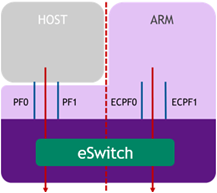
\includegraphics[]{separated-mode.png}
    \caption{separated-mode}
    \label{fig:sep-mode}
\end{figure}

In modalità embedded, le risorse e le funzionalità dell'interfaccia di rete sono di proprietà e 
controllate interamente dalla DPU e dallo stack software. 
Una funzione di rete è ancora esposta all'host, ma ha privilegi limitati.

In particolare, il driver sul lato host può essere caricato solo dopo il caricamento del driver
 sul lato embedded. 
La DPU controlla le risorse e le funzionalità dell'interfaccia di rete, ciò significa che il 
traffico da e verso l'interfaccia host 
arriva e passa sempre attraverso la DPU in entrambe le direzioni. 
In modalità embedded, ci sono due modi per passare il traffico alle interfacce host, utilizzando 
i rappresentanti per inoltrare il traffico all'host, 
in modo che ogni pacchetto da e verso l'host venga gestito anche dall'interfaccia di rete sul lato del processore Arm embedded, oppure
 inviare le regole allo switch incorporato, che accelera e scarica il flusso per ottenere prestazioni di velocità di linea.
\begin{figure}[H]
    \centering
    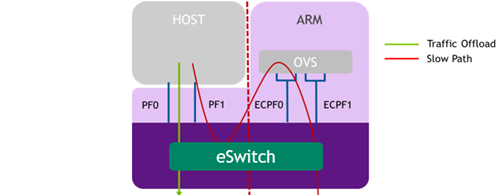
\includegraphics[]{embedded-mode.png}
    \caption{embedded-mode}
    \label{fig:emb-mode}
\end{figure}

Ora analizziamo un po' più a fondo i tipi e gli usi specifici delle accelerazioni e degli offload che Bluefield e DOCA possono offrire. 

\subsubsection{Crittografia}

La crittografia è un aspetto importante delle architetture di sicurezza. Che si tratti di archiviazione o di trasmissione di dati, il lavoro di calcolo richiesto per eseguire le funzioni di crittografia e decrittografia può consumare rapidamente la maggior parte dei cicli della CPU a velocità di throughput dei data center.
Le DPU Bluefield forniscono motori di accelerazione hardware dedicati per eseguire la crittografia e la decrittografia simmetriche utilizzate per la sicurezza del transito basato sulla rete. 
Si noti che spostando la funzione di crittografia alla DPU, l'host non ha più bisogno di una CPU generica per eseguire queste operazioni e può lasciare che la DPU gestisca la crittografia di sicurezza come parte della propria funzione di rete, alleggerendo la responsabilità dell'applicazione.

Analogamente, con gli acceleratori di crittografia e decrittografia, le DPU Bluefield possono accelerare e scaricare il duro lavoro di crittografia e decrittografia per le connessioni di sicurezza del livello di trasporto. 
Rispetto a IPsec, TLS fornisce un socket sicuro a un'applicazione invece di un tunnel sicuro dedicato tra due endpoint IP. 
TLS dipende da diverse operazioni a chiave pubblica durante l'handshake e sfrutta altri motori di accelerazione integrati per scaricare queste funzioni e consentire velocità di connessione al secondo più elevate.

Come abbiamo accennato per TLS, Bluefield contiene un motore di accelerazione delle operazioni a chiave pubblica per scaricare le operazioni di firma a chiave pubblica OpenSSL. 
Questo include le operazioni di firma e verifica RSA a 2048 e 4096 bit, gli algoritmi di 
firma Diffie-Hellman, DSA ed EC-DSA. Include anche un vero generatore di numeri casuali per 
garantire che i numeri casuali siano veramente casuali e non generati algoritmicamente.


Questo motore di accelerazione può contribuire a ridurre il sovraccarico per i casi d'uso, 
come ad esempio un server Web Https che sfrutta TLS; infatti potrebbe ridurre il sovraccarico della
configurazione della connessione TLS e dell'handshaking in cui avvengono le operazioni 
di firma e verifica.

\subsubsection{Motore Regex}
Le espressioni regolari hanno un'ampia gamma di casi d'uso per i software di sicurezza di rete, come i firewall di nuova generazione o il rilevamento delle intrusioni. 
Il principale collo di bottiglia e la maggior parte del tempo di elaborazione vengono spesi per la per la corrispondenza dei pattern per le minacce a livello di applicazione. 
Al di là delle intestazioni statiche dei pacchetti, la maggior parte del traffico di rete è 
costituita dal payload dei dati, che varia in termini di dimensioni o lunghezza. 
Le minacce possono essere presenti in qualsiasi punto del payload di un pacchetto e diventa 
difficile cercare in modo efficiente nel payload di ogni pacchetto una serie di minacce ad alta velocità di trasmissione dei dati. Bluefield fornisce un motore di espressioni regolari per accelerare
e scaricare l'elaborazione della corrispondenza dei pattern per i payload dei pacchetti di rete.
Questo riduce in modo significativo il sovraccarico della CPU per accelerare applicazioni e casi d'uso quali
prevenzione delle intrusioni, bilanciatori di carico stateful, protezione DDoS e firewall per applicazioni web.

%_______________________________________________________________________________________
\subsection{DOCA}

Nvidia DOCA è un insieme di software che comprende librerie, driver, runtime, ecc. che consente di utilizzare l'accelerazione DPU. 
Doca è simile per molti aspetti a CUDA.
CUDA è per molti versi una piattaforma per consentire l'accelerazione del calcolo tramite GPU e,
allo stesso modo, DOCA vuole essere la piattaforma o il mezzo per consentire  di sfruttare i 
diversi tipi di acceleratori di calcolo delle DPU BlueField.
La strategia finale è quella di liberare i cicli della CPU X 86 di uso generale in modo che 
possano essere utilizzati in modo più efficiente per le applicazioni di calcolo che svolgono
 il lavoro più interessante.
A seconda dell'applicazione e dei suoi requisiti di I/O, potrebbe esserci una quantità
considerevole di tempo e di sforzi della CPU spesi in operazioni generali come l'ingresso 
e l'uscita dei dati dall'applicazione e dal sistema, o per routine e compiti di calcolo comuni 
per i quali l'implementazione hardware è molto più ottimizzata rispetto all'implementazione 
per un processore X 86 di uso generale. DOCA e le DPU sono progettati per fornire una piattaforma
flessibile che consenta di trasferire o scaricare alcuni di questi compiti ai core ARM,
oppure di utilizzare uno dei numerosi motori di accelerazione hardware dedicati per gestire
il lavoro computazionalmente difficile richiesto dalle moderne soluzioni di I/O ad alta velocità.

Questa(\ref{fig:doca}) è un'illustrazione dei singoli componenti software di DOCA e di come sono impilati 
insieme e dipendono l'uno dall'altro. Le applicazioni in alto non sono in realtà componenti
software, ma descrivono i principali pilastri o casi d'uso di DOCA e delle DPU.
\begin{figure}[H]
    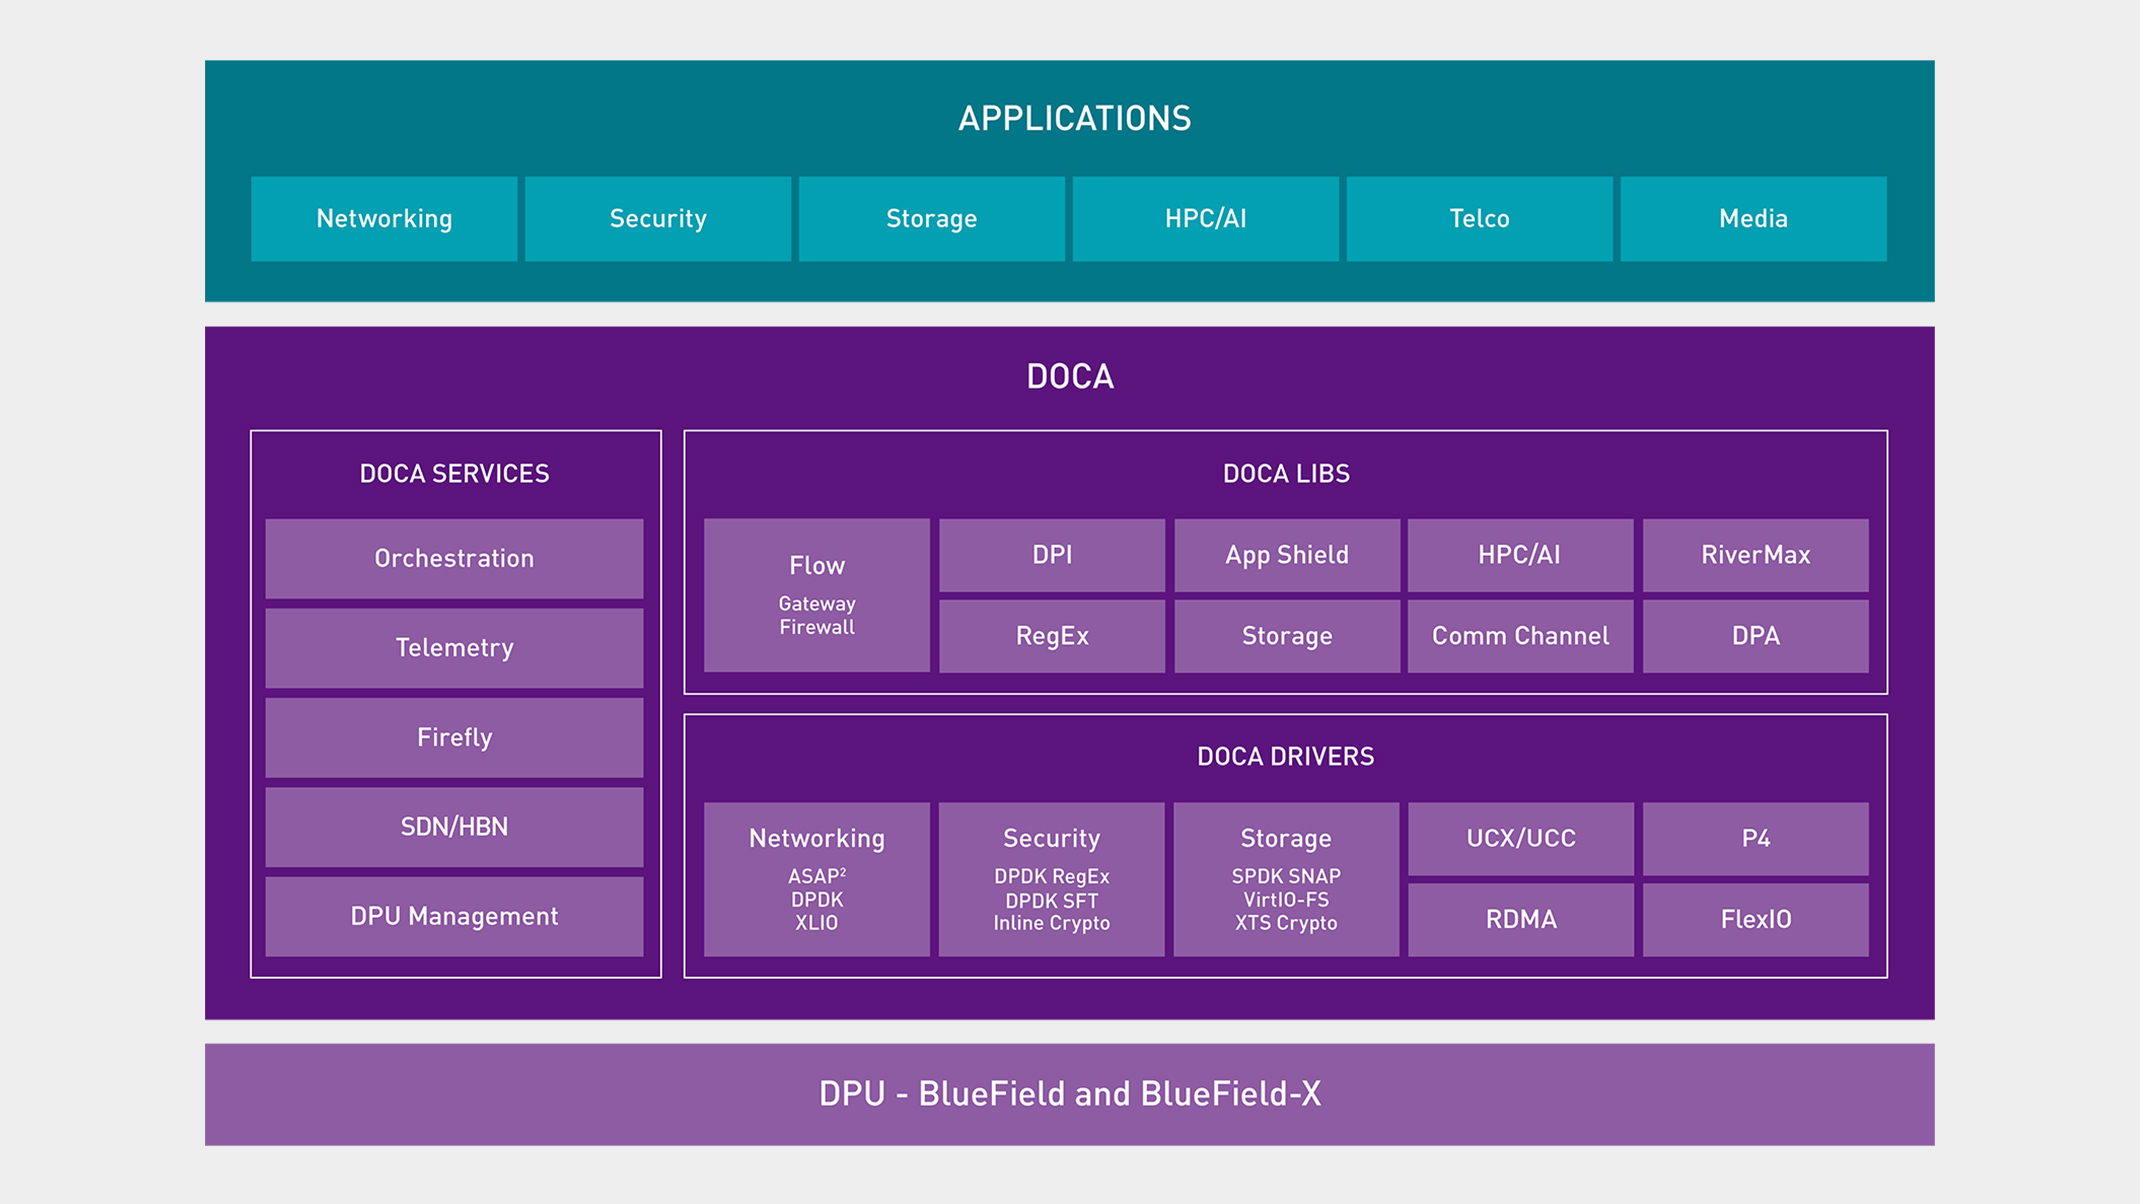
\includegraphics[width=\textwidth]{doca}
    \caption{doca}
    \label{fig:doca}
\end{figure}

\subsubsection*{Libreria DPI}

Nelle librerie DOCA, si possono notare alcune cose come DPI o Deep Packet Inspection 
sono sovrapposte a regex. DOCA fornisce una libreria DPI che sfrutta le librerie runtime regex.

Diamo una rapida occhiata a ciò che fornisce 
la libreria DPI di DOCA. La libreria DPI fornisce un framework per identificare facilmente gli 
schemi nel payload del traffico di rete. La libreria DPI combina diverse funzioni accelerate dalla
DPU, oltre a fornire funzionalità di pre-elaborazione o parsing dei pacchetti e routine di 
post elaborazione, in modo che gli sviluppatori di applicazioni possano scrivere più rapidamente 
applicazioni che agiscono in base al contenuto del traffico di rete al di là delle intestazioni 
dei pacchetti.

Queste librerie sono scritte nel linguaggio di programmazione C. 
Senza la libreria DPI di Doca, gli sviluppatori di applicazioni dovrebbero scrivere e 
mantenere tutto il codice per analizzare le intestazioni dei pacchetti.

%\subsubsection*{Compilatore DPI}


%_______________________________________________________________________________________
\chapter{Configurazione}

In questo capitolo vedremo nel dettaglio come configurare tutto il necessario per poter 
utilizzare la scheda Bluefield.Iniziando dalla scheda stessa, dall'installazione dei suoi driver
e anche le instruzioni necessarie per poter accedere alla SmartNic.
Poi passeremo alla descrizione dell'installazione del kit di sviluppo DOCA.
E infine gli ultimi passaggi richiesti per poter eseguire un'applicazione sulla DPU, che sono:
la creazione delle Scalable Functions e la configurazione dell'open virtual switch.
%_______________________________________________________________________________________
\section{Installazione Bluefield}
Per installare i driver della scheda Bluefield abbiamo seguito una guida(\cite{install bluefield }) che riassume i 
pricipali passaggi presenti anche nella documentazione.
\subsubsection*{Scaricare i driver}
\begin{verbatim}
# cd /opt   
# wget http://www.mellanox.com/downloads/ofed/MLNX_OFED-5.3-1.0.0.1
/MLNX_OFED_LINUX-5.3-1.0.0.1-ubuntu20.04-x86_64.tgz
\end{verbatim}
\subsubsection*{Decomprimere ed installare} 

\begin{verbatim}
# tar -xzvf MLNX_OFED_LINUX-5.3-1.0.0.1-ubuntu20.04-x86_64.tgz 
# cd MLNX_OFED_LINUX-5.3-1.0.0.1-ubuntu20.04-x86_64 
# ./mlnxofedinstall --auto-add-kernel-support --without-fw-update 
\end{verbatim}
\subsubsection*{Riavvia openibd di MLNX\_OFED: }
\begin{verbatim}
# /etc/init.d/openibd restart
Unloading HCA drvier:                [ OK ]
Loading HCA driver and Access Layer: [ OK ]
\end{verbatim}
Per impostazione predefinita, lo script di installazione installerà anche rshim .
Rshim permette la comunicazione del  sistema host  
con lo SmartNIC tramite Ethernet. In altre parole, il livello rshim crea interfacce
fittizie con indirizzi IP locali sia sull'host che sul Bluefield, quindi possiamo 
facilmente entrare in SSH nella NIC dall'host. 


\subsubsection*{Abilitare rshim e avviarlo } 
\begin{verbatim}
# systemctl enable rshim
# systemctl start rshim
\end{verbatim}
Controllare lo stato  
\begin{verbatim}
# systemctl status rshim
rshim.service - rshim driver for BlueField SoC
Loaded: loaded (/lib/systemd/system/rshim.service; enabled;...)
Active: active (running) since Wed 2021-04-07 20:56:36 EDT; 19min ago
Docs: man:rshim(8)
Main PID: 438156 (rshim)
Tasks: 6 (limit: 618619)
Memory: 1.8M
CGroup: /system.slice/rshim.service
438156 /usr/sbin/rshimApr 07 20:56:36 node-0.cslev-qv95721.k8s-
dataplane-pg0.clemson.cloudlab.us systemd[1]: 
Starting rshim driver for BlueField SoC...
\end{verbatim}

\subsubsection*{Acceedere alla Bluefield tramite rshim}
Per prima cosa, dobbiamo impostare un indirizzo IP per l'interfaccia host tmfifo\_net0 di rshim 
che è già visibile dopo l'installazione di rshim stesso.Per farlo 
bisogna modificare il file /etc/netplan/01-netcfg.yaml
aggiungendo le ultime 3 righe presentate nell'esempio seguente: 
\begin{verbatim}
sudo cat /etc/netplan/01-netcfg.yaml
# This file describes the network interfaces available on your system
# For more information, see netplan(5).
network:
  version: 2
  renderer: networkd
  ethernets:
    eno1:
      dhcp4: yes
    tmfifo_net0:
  	  addresses: [192.168.100.1/24]
      dhcp4: false
\end{verbatim}

\subsubsection*{Riavvio della rete}

\begin{verbatim}
systemctl restart systemd-networkd
\end{verbatim}
\subsubsection*{Test}
Se tutto va bene, possiamo provare a eseguire il ping di Bluefield-2 .
\begin{verbatim}
# ping -I tmfifo_net0 192.168.100.2 -c2
\end{verbatim}
\subsubsection*{Connessione}
\begin{verbatim}
ssh ubuntu@192.168.100.2
Password: ubuntu
\end{verbatim}

%______________________________________________________________________________________________

\section{Installazione Doca(v.1.2)}
Per installare DOCA(la versione 1.2) abbiamo seguito i passaggi presenti  nella
documentazione DOCA SDK (\cite{doca doc url filter}). Si può installare DOCA tramite 
NVIDIA SDK Manager che include tutti i pacchetti necessari per l'host e per la BlueField.
Oppure si può procedere con l'installazione manuale dei pacchetti.
\subsubsection*{Installare DOCA sull'host}
Scaricare il pacchetto DOCA Tools dalla sezione dei file di installazione per l'host.\\
Decomprimere la repository deb ed eseguire: 
\begin{verbatim}
sudo dpkg -i doca-host-repo-ubuntu<version>_amd64.deb
\end{verbatim}
Eseguire l'apt update
\begin{verbatim}
sudo apt-get update
\end{verbatim}
Eseguire  apt install per DOCA SDK, DOCA runtime, DOCA tools.
\begin{verbatim}
sudo apt install doca-sdk
sudo apt install doca-runtime
sudo apt install doca-tools
\end{verbatim}
\subsubsection*{Installare DOCA sulla Bluefield}


Scaricare i pacchetti DOCA SDK, DOCA Runtime e DOCA Tools dalla sezione dei file di installazione.\\
Copiare la repository dep sulla Bluefield.
\begin{verbatim}
sudo scp -r doca-repo-aarch64-ubuntu2004-local_<version>_arm64.deb 
ubuntu@192.168.100.2:/tmp/
\end{verbatim}
Decomprimere la repository deb.
\begin{verbatim}
sudo dpkg -i doca-repo-aarch64-ubuntu2004-local_<version>_arm64.deb
\end{verbatim}
Eseguire l'apt update
\begin{verbatim}
sudo apt-get update
\end{verbatim}
Eseguire  apt install per DOCA SDK, DOCA runtime, DOCA tools.
\begin{verbatim}
sudo apt install doca-sdk
sudo apt install doca-runtime
sudo apt install doca-tools
\end{verbatim}
%_______________________________________________________________________________________
\section{Esecuzione di un'applicazione su BlueField}

In questa sezione vedremo come poter eseguire un'applicazione sulla scheda Bluefield.
In particolare ci focalizeremo sull'applicazione di esempio URL-filter presente sulla documentazione Doca 1.2 \cite{doca doc url filter}.
Evidenziando i passaggi necessari affinché tutto funzioni.\\
a) Per ricompilare l'appicazione
\begin{lstlisting}[ backgroundcolor=\color{LightYellow},frame=none,stepnumber=0]
cd /opt/mellanox/doca/examples/url_filter/src
meson /tmp/build 
ninja -C /tmp/build
\end{lstlisting}
Il processo di compilazione dipende dalla variabile di ambiente PKG\_CONFIG\_PATH per individuare il file Librerie DPDK. Se la variabile è stata danneggiata accidentalmente e la compilazione non riesce, eseguire il file seguente comando: 
\begin{lstlisting}[ backgroundcolor=\color{LightYellow},frame=none,stepnumber=0]
export PKG_CONFIG_PATH=$PKG_CONFIG_PATH:/opt/mellanox/dpdk/lib/aarch64-linux-gnu/pkgconfig
\end{lstlisting}
b) L'esempio URL-filter si basa sulle librerie DPDK. Pertanto, l'utente deve fornire i flag DPDK e allocare pagine enormi. 
\begin{lstlisting}[ backgroundcolor=\color{LightYellow},frame=none,stepnumber=0]
echo 2048 > /sys/kernel/mm/hugepages/hugepages-2048kB/nr_hugepages
\end{lstlisting}
oppure
\begin{lstlisting}[ backgroundcolor=\color{LightYellow},frame=none,stepnumber=0]
echo '2048' | sudo tee -a /sys/kernel/mm/hugepages/hugepages-2048kB/nr_hugepages
\end{lstlisting}
c) Assicurarsi che il motore regex sia attivo
\begin{lstlisting}[ backgroundcolor=\color{LightYellow},frame=none,stepnumber=0]
systemctl status mlx-regex
\end{lstlisting}
Se lo stato è inattivo (Active: failed)
\begin{lstlisting}[ backgroundcolor=\color{LightYellow},frame=none,stepnumber=0]
systemctl start mlx-regex
\end{lstlisting}
d) Per eseguire l'applicazione
\begin{lstlisting}[ backgroundcolor=\color{LightYellow},frame=none,stepnumber=0]
/opt/mellanox/doca/examples/url_filter/bin/doca_url_filter -a 0000:03:00.0,class=regex -a auxiliary:mlx5_core.sf.4,sft_en=1 -a auxiliary:mlx5_core.sf.5,sft_en=1 -c3 -- -p
\end{lstlisting}

\subsection{Scalabale Function}
Una nota nella guida ci ricorda che bisogna abilitare le Scalable Function(SF). 
In questa sottosezione vedremo cosa sono e le istruzioni da eseguire per attivarle.
\cite{doca doc scalable function }
Le funzioni scalabili (SF), o sottofunzioni, sono molto simili alle funzioni virtuali (VF) che fanno
parte dell'interfaccia SR-IOV (Single Root I/O Virtualization).
La virtualizzazione degli I/O è una delle le funzionalità chiave utilizzate oggi nei data center.
SR-IOV consente a un dispositivo, ad esempio una scheda di rete, di separare l'accesso alle risorse
 tra varie funzioni hardware PCIe. Queste funzioni sono costituite da questi tipi:
\begin{itemize}
    \item Una funzione fisica PCIe (PF). Questa funzione è la funzione principale del dispositivo e 
    annuncia le funzionalità SR-IOV del dispositivo. 
    \item Una o più funzioni virtuali PCIe. Ogni VF è associato al file PF del dispositivo. 
    Un VF condivide una o più risorse fisiche del dispositivo, ad esempio una memoria e una porta 
    di rete, con PF e altre VF nel dispositivo. 

\end{itemize}    
Per utilizzare le capacità delle VF nella scheda BlueField, vengono utilizzati le SF.
Una SF è una funzione leggera che ha una funzione PCIe padre su cui è distribuita. 
La SF, quindi, ha accesso alle capacità e alle risorse della sua funzione principale PCIe 
e ha le proprie capacità funzionali e le proprie risorse. Ciò significa che una SF avrà anche le sue code dedicate
(ad esempio, txq, rxq).
Le SF coesistono con le funzioni virtuali PCIe SR-IOV (sull'host) ma non richiedono l'
abilitazione PCIe SR-IOV. 
Una SF condivide le risorse a livello PCIe con altre SF e/o con la sua funzione PCIe principale.  
\begin{figure}[H]
    \centering
    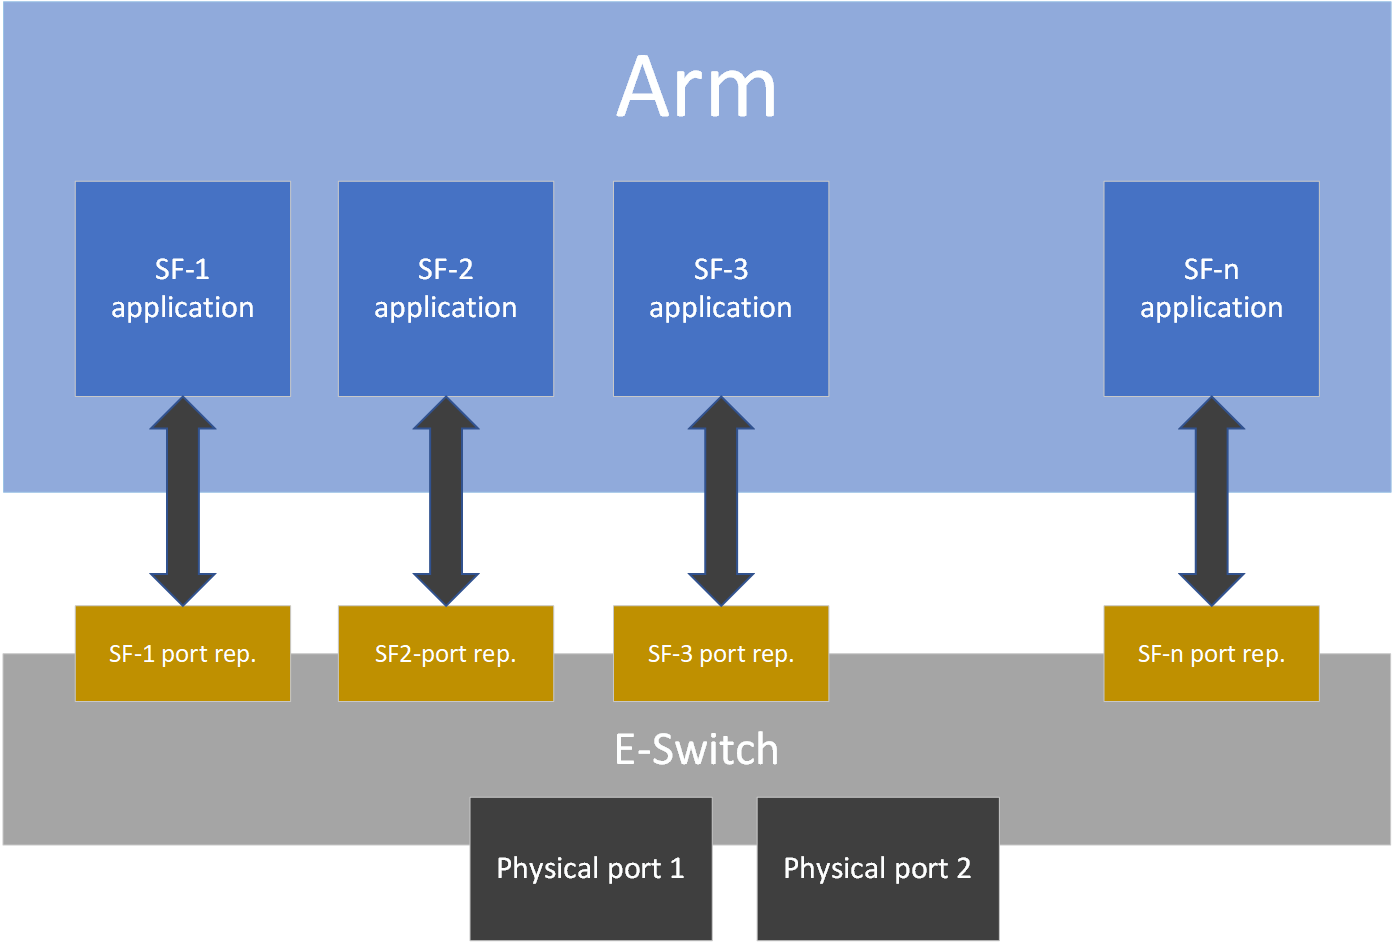
\includegraphics[scale=0.3]{scalable-functions-illustration.png}
    \caption{Scalable functions}
    \label{fig:sf}
\end{figure}


\subsubsection{Creare e configurare le SF}
a) Creare le SF.
\begin{lstlisting}[ backgroundcolor=\color{LightYellow},frame=none,stepnumber=0]
/opt/mellanox/iproute2/sbin/mlxdevm port add pci/0000:03:00.0 flavour pcisf pfnum 0 sfnum 4
/opt/mellanox/iproute2/sbin/mlxdevm port add pci/0000:03:00.0 flavour pcisf pfnum 0 sfnum 5 
\end{lstlisting}
Per vedere gli indici delle SF create:
\begin{lstlisting}[ backgroundcolor=\color{LightYellow},frame=none,stepnumber=0]
/opt/mellanox/iproute2/sbin/mlxdevm port show
\end{lstlisting}
Esempio
\begin{lstlisting}[ backgroundcolor=\color{LightYellow},frame=none,stepnumber=0]
pci/0000:30:00.0/229409: type eth netdev en3f0pf0sf4 flavour pcisf controller 0 pfnum 0 sfnum 4 
   function:
	hw_addr 00:00:00:00:00:00 state inactive opstate detached roce true max_uc_macs 128 trust off
pci/0000:30:00.0/229410: type eth netdev en3f0pf0sf5 flavour pcisf controller 0 pfnum 0 sfnum 5
   function:
	hw_addr 00:00:00:00:00:00 state inactive opstate detached roce true max_uc_macs 128 trust off
\end{lstlisting}
b) Configurare l'indirizzo MAC e attivare le SF create:
\begin{lstlisting}[ backgroundcolor=\color{LightYellow},frame=none,stepnumber=0]
/opt/mellanox/iproute2/sbin/mlxdevm port function set pci/0000:03:00.0/229409 hw_addr 02:25:f2:8d:a2:4c trust on state active
/opt/mellanox/iproute2/sbin/mlxdevm port function set pci/0000:03:00.0/229410 hw_addr 02:25:f2:8d:a2:5c trust on state active
\end{lstlisting}
c) Per separare la SF dal driver di configurazione predefinito e associarlo all'attuale driver SF 
\begin{lstlisting}[ backgroundcolor=\color{LightYellow},frame=none,stepnumber=0]
echo mlx5_core.sf.4  > /sys/bus/auxiliary/drivers/mlx5_core.sf_cfg/unbind
echo mlx5_core.sf.4  > /sys/bus/auxiliary/drivers/mlx5_core.sf/bind
\end{lstlisting}
\begin{lstlisting}[ backgroundcolor=\color{LightYellow},frame=none,stepnumber=0]
echo mlx5_core.sf.5  > /sys/bus/auxiliary/drivers/mlx5_core.sf_cfg/unbind
echo mlx5_core.sf.5  > /sys/bus/auxiliary/drivers/mlx5_core.sf/bind
\end{lstlisting}
Usando \textsl{ifconfig} , si può vedere che ne sono stati aggiunte 2 interfacce di rete: \textsl{en3f0pf0sf4} e \textsl{en3f0pf0sf5} per le due rispettive porte SF rappresentanti. 



\subsection{Open virtual switch(ovs)}
Inoltre la documentazione ci dice che l'esecuzione di un'applicazione sulla DPU 
richiede la configurazione di OVS. Creando una SF, viene creato anche un rappresentante 
SF per OVS che ha il nome \textsl{en3f0pf*sf*} . Pertanto, ogni rappresentante deve esserlo collegato 
al bridge OVS corretto. \\
Ecco i comandi per una corretta configurazione di ovs:
\begin{lstlisting}[ backgroundcolor=\color{LightYellow},frame=none,stepnumber=0]
ovs-vsctl add-br sf_bridge1
ovs-vsctl add-br sf_bridge2
ovs-vsctl add-port sf_bridge1 pf0hpf
ovs-vsctl add-port sf_bridge1 en3f0pf0sf4
ovs-vsctl add-port sf_bridge2 p0
ovs-vsctl add-port sf_bridge2 en3f0pf0sf5 
\end{lstlisting}
Di seguito viene mostrato il comando per una panoramica del database Open vSwitch.
E anche una rappresentazione grafica(figura \ref{fig:ovs}).
\begin{lstlisting}[ backgroundcolor=\color{LightYellow},frame=none,stepnumber=0]
sudo ovs-vsctl show
d3a1e07e-43a0-45a8-bbc4-da75864bc5bc
    Bridge sf_bridge2
        Port en3f0pf0sf5
            Interface en3f0pf0sf5
        Port p0
            Interface p0
        Port sf_bridge2
            Interface sf_bridge2
                type: internal
    Bridge sf_bridge1
        Port en3f0pf0sf4
            Interface en3f0pf0sf4
        Port sf_bridge1
            Interface sf_bridge1
                type: internal
        Port pf0hpf
            Interface pf0hpf
    ovs_version: "2.15.1"

\end{lstlisting}
\begin{figure}[h]
    \centering
    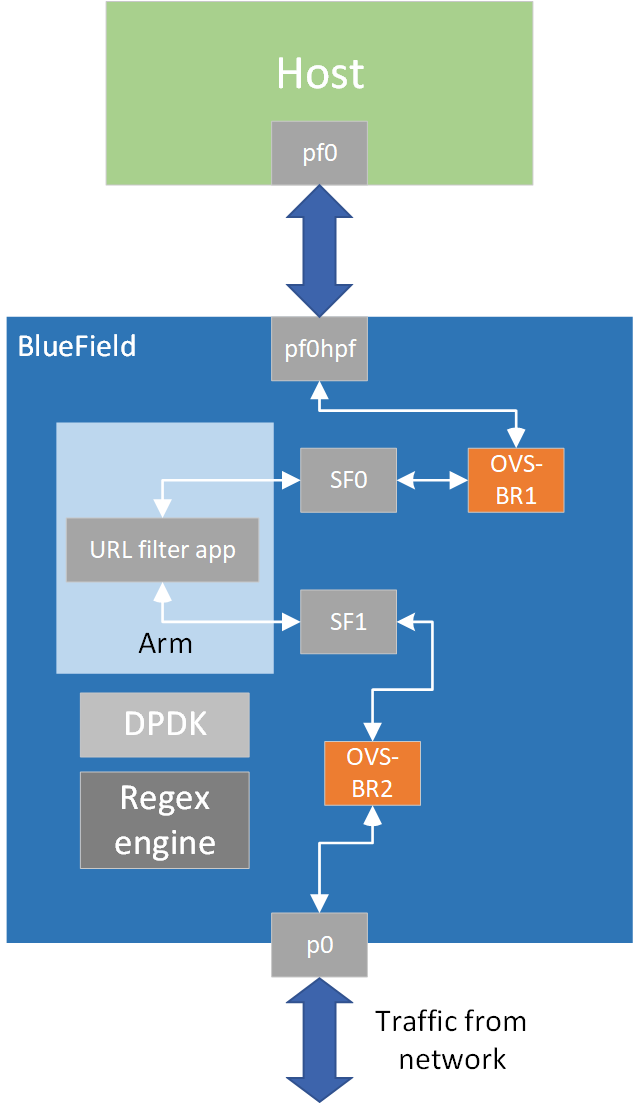
\includegraphics[scale=0.48]{system-design-diagram-url-filter.png}
    \caption{Schema di progettazione del sistema}
    \label{fig:ovs}
\end{figure}

%_________________________________________________________________________________________________
\chapter{Applicazione}
In questo capitolo vedremo in dettaglio tutti gli aspetti dell'applicazione.
Abbiamo detto che il programma dovrà effettuare l'operazione di bilanciamento del 
carico (Load balancing), cioè distribuire i pacchetti su diversi server.
Per fare ciò, dobbiamo scegliere dei criteri in base ai quali effettuare la scelta di instradamento.
Nel nostro caso la scelta verrà effettuata in base allo user agent del client.
Un possibile utilizzo per questa applicazione è quello di instradare le richieste che provengono
da uno smartphone su un server che contiente risorse specifiche per quel dispositivo e invece
le richieste che provengono da un computer su un altro server.
Una volta identificato la provenienza di una richiesta e calcolato la porta di uscita su cui 
instradarla, salveremo queste informazioni in una struttura dati per evitare di dover processare
nuovamente un pacchetto del quale sappiamo già la destinazione.
Per fare questo lavoro sfrutteremo il motore Regex della scheda Bluefield, il quale filtrerà i
pacchetti in base a specifiche regole in input.
Abbiamo parlato di bilanciamento di carico(\ref{chapter:load balancing}), 
di user agent(\ref{chapter:http}),di strutture dati(\ref{chapter:hash table}) e
di regole di filtraggio(\ref{chapter:suricata}). 
Questi sono tutte gli argomenti delle prossime sezioni. 
Infine vedremo alcune parti dell'implementazione(\ref{chapter:implementazione}) con principali funzioni del codice.


%_________________________________________________________________________________________________
\section{Load balancing}
\label{chapter:load balancing}
Di seguito è riportato un'estratto dal libro "Reti di calcolatori e internet. Un approccio top-down."
\cite{Reti di calcolatori} che per l’appunto parla di bilanciamento di carico.\\
Un data center per cloud computing, come quelli di Google o Microsoft, fornisce parallelamente
molte applicazioni come la ricerca sul Web, l’e-mail e le applicazioni
video. Per supportare le richieste da client esterni, a ogni applicazione è associato un
indirizzo IP visibile pubblicamente al quale i client inviano le loro richieste e dal qua-
le ricevono le risposte. All’interno del data center le richieste esterne vengono prima
dirette a un load balancer (bilanciatore di carico) il cui compito è di distribuire le
richieste agli host, bilanciando il lavoro in funzione del loro carico corrente. Un gran-
de data center ha tipicamente molti load balancer, ognuno dei quali è dedicato a un
particolare insieme di applicazioni. Un load balancer di questo tipo è spesso chiamato
“switch di livello 4” poiché prende decisioni sulla base del numero di porta di destinazione
(livello 4) e dell’indirizzo IP di destinazione del pacchetto. Il load balancer
quando riceve una richiesta per una particolare applicazione, la inoltra a uno degli
host che gestisce tale applicazione. Un host può quindi richiedere i servizi di altri
host che lo aiutino a processare la richiesta. L’host, quando finisce di elaborare la richiesta,
invia la risposta al load balancer che a sua volta la ritrasmette al client esterno

\begin{figure}[h]
    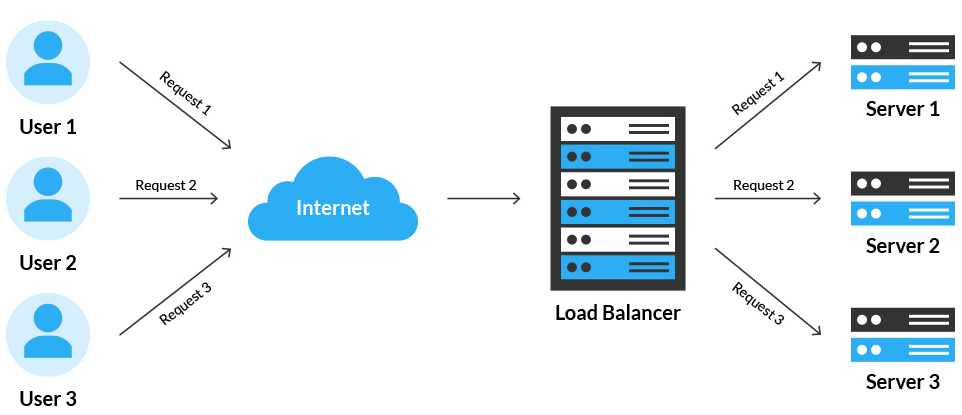
\includegraphics[width=\textwidth]{load-balancing.jpg}
    \caption{Load balancing}
    \label{fig:load-balancer}
\end{figure}

Il bilanciamento del carico può essere eseguito a vari livelli nel modello di 
riferimento OSI (Open Systems Interconnection) per il networking.
Quindi oltre al bilanciamento di carico al livello 4 di cui si è parlato prima, possiamo bilanciare
il carico al livello 7 cioè al livello applicazione.
Quest'ultimo si occupa del contenuto effettivo di ciascun messaggio. 
I sistemi di bilanciamento del carico di livello 7 instradano il traffico di rete in un modo molto
più sofisticato rispetto ai sistemi di bilanciamento del carico di livello 4.
Prendono una decisione di bilanciamento del carico in base al contenuto
del messaggio (lo user agent, ad esempio).
%_________________________________________________________________________________________________
\section{Protocollo HTTP }
\label{chapter:http}
Il nostro load balancer opererà al livello 7 della pila OSI, prendendo decisioni in base ai campi
del protocollo HTTP del pacchetto,quindi vediamo un po' di dettagli su questo protocollo.
\cite{Reti di calcolatori}\\
Hypertext Transfer Protocol (HTTP) è un metodo per codificare e trasportare informazioni tra un client (come un browser Web) e un server Web . HTTP è il protocollo principale per la trasmissione di informazioni su Internet.

Le informazioni vengono scambiate tra client e server sotto forma di documenti ipertestuali, da cui HTTP prende il nome. L'ipertesto è un testo strutturato che utilizza collegamenti logici, o collegamenti ipertestuali , tra nodi contenenti testo. I documenti ipertestuali possono essere manipolati utilizzando l'Hypertext Markup Language (HTML). Utilizzando HTTP e HTML, i client possono richiedere diversi tipi di contenuto (come testo, immagini, video e dati dell'applicazione) dal Web e dai server delle applicazioni che ospitano il contenuto.

HTTP segue un paradigma richiesta-risposta in cui il client effettua una richiesta e il server emette una risposta che include non solo il contenuto richiesto, ma anche informazioni di stato rilevanti sulla richiesta. Questo design autonomo tiene conto della natura distribuita di Internet, in cui una richiesta o una risposta potrebbe passare attraverso molti router intermedi e server proxy. Consente inoltre ai server intermedi di eseguire funzioni a valore aggiunto come bilanciamento del carico, memorizzazione nella cache, crittografia e compressione.


HTTP è un protocollo a livello di applicazione e si basa su un protocollo a livello di rete sottostante come il TCP (Transmission Control Protocol) per funzionare. 


\subsubsection{Intestazione richiesta Http}
Di seguito vediamo un'esempio di un'intestazione di una richiesta Http che potrebbe arrivare
al load balancer.

\begin{table}[ht]
    \centering
    \caption*{\textbf{Esempio 4.1} Intestazione di una richiesta http}
    \begin{tabular}{ |l|c|}
        \hline
        GET /ethereal-labs/lab2-1.html HTTP/1.1   \\ 
        {Host}: gaia.cs.umass.edu   \\  
        {User-Agent}: Mozilla/5.0 (Windows; U; Windows NT 5.1; en-US; rv:1.0.2) \\Gecko/20021120 Netscape/7.01\\
        {Accept}: text/xml,application/xml,application/xhtml+xml,text/html;q=0.9,\\text/plain;q=0.8,video/x-mng,image/png,image/jpeg,\\image/gif;q=0.2,text/css,*/*;q=0.1\\ 
        {Accept-Language}: en-us, en;q=0.50\\ 
        {Accept-Encoding}: gzip, deflate, compress;q=0.9\\ 
        {Accept-Charset}: ISO-8859-1, utf-8;q=0.66, *;q=0.66\\ 
        {Keep-Alive}: 300\\ 
        {Connection}: keep-alive\\   
        \hline
    \end{tabular}

\end{table}

Un campo che ci interessa particolarmente è lo User-Agent,
tramite il quale possono essere date delle informazioni più o meno approfondite riguardo al 
dispositivo che effettua la richiesta di rete.Tali informazioni possono essere usate, ad esempio, 
per inviare determinati elementi solo a quei browser che possono effettivamente processarli.
Di seguito possiamo vedere due User-Agent diversi. Il primo (esempio 4.2) ci dice 
che la richiesta è stata effettuta da un dispositivo con un sistema operativo Windows.
Il secondo (esempio 4.3) ci dice 
che la richiesta è stata effettuta da un dispositivo con un sistema operativo Android.
\begin{table}[ht]
    \centering
    \caption*{\textbf{Esempio 4.2} Richieta effettuato da un computer desktop}
    \begin{tabular}{ |l|c|}
        \hline
        {User-Agent}: Mozilla/5.0 (Windows; U; Windows NT 5.1; en-US; rv:1.0.2) \\Gecko/20021120 Netscape/7.01\\
         
        \hline
    \end{tabular}

\end{table}


\begin{table}[ht]
    \centering
    \caption*{\textbf{Esempio 4.3} Richieta effettuato da un computer desktop}
    \begin{tabular}{ |l|c|}
        \hline
        {User-Agent}: Mozilla/5.0 (Linux; Android 12) AppleWebKit/537.36 \\(KHTML, like Gecko) Chrome/103.0.5060.71 Mobile Safari/537.36\\
        \hline
    \end{tabular}

\end{table}


%_________________________________________________________________________________________________
\section{Regole Suricata}
\label{chapter:suricata}
Per poter utilizzare l'acceleratore regex della scheda Bluefield bisogna caricare le firme. 
Questa operazione viene fatta dal compilatore DPI che compila un file di firme e lo carica nel 
motore regex.
Il compilatore DOCA DPI ha un supporto limitato per il formato Suricata. 
quindi in questa sezione vedremo come scrivere delle regole in formato Suricata.\\
Una regola/firma è composta da quanto segue:
\begin{itemize}
    \item L'azione, che determina ciò che accade quando la firma ha una corrispondenza 
    \item L'intestazione, che definisce il protocollo, gli indirizzi IP, le porte e la direzione della regola.
    \item Le opzioni della regola, che definiscono le specifiche della regola.
\end{itemize}

\begin{table}[ht]
    \centering
    \caption*{\textbf{Esempio 4.4} Regola Suricata}
    \begin{tabular}{ |l|c|}
        \hline
        alert tcp \$ EXTERNAL\_NET any -> 10.200.0.0/24 80 \\
        (msg:"WEB-IIS CodeRed v2 root.exe access"; flow:to\_server,established;\\
         uricontent:"/root.exe"; nocase; classtype:web application-attack; \\
         reference:url,www.cert.org/advisories/CA-2001 19.html; sid:1255; rev:7;)\\
        \hline
    \end{tabular}
\end{table}

Per una migliore comprensione analizziamo le singole parti della regola nell'esempio 4.1.

\begin{itemize}[topsep=10pt, noitemsep]


    \item[--] {alert}  : dice di segnalare questo comportamento come un avviso. Ci sono anche altri tipi di azione come per esempio: -\textit{pass} che interrompe l'ulteriore ispezione del pacchetto;
    \textit{drop} che elimina il pacchetto e genera un avviso e
    \textit{reject} che invia un errore ICMP  al mittente del pacchetto corrispondente.

    \item[--] tcp : significa che questa regola si applicherà solo al traffico in TCP. Si posso scegliere anche altri protocolli come udp,icmp,http,ftp,tls,smb,dns...(la lista completa è presente sulla documentazione \cite{documentazione Suricata}).

    \item[--] \$EXTERNAL\_NET : questa è una variabile definita in Suricata. Per impostazione predefinita, la variabile HOME\_NET è definita come qualsiasi IP all'interno di questi intervalli: 192.168.0.0/16,10.0.0.0/8,172.16.0.0/12 e EXTERNAL\_NET è definito come qualsiasi IP al di fuori di questi intervalli. È possibile specificare gli indirizzi IP specificando un singolo IP come 10.200.0.0, un intervallo IP CIDR come 192.168.0.0/16 o un elenco di IP come [192.168.0.0/16,10.0.0.0/8].

    \item[--] any : in questo contesto, significa "da qualsiasi porta di origine", quindi c'è una freccia '->' che significa "una connessione a" (non c'è un operatore '<-', ma puoi semplicemente capovolgere gli argomenti. È possibile utilizzare l'operatore '<>' per indicare che la direzione della connessione è irrilevante per questa regola), poi c'è un intervallo IP che indica l'indirizzo IP di destinazione e infine la porta. Puoi indicare un intervallo di porte usando i due punti come 0:1024 che significa 0-1024.
    
    \item[--] msg : è una direttiva che imposta semplicemente il messaggio che verrà inviato nel caso venga rilevato un traffico corrispondente.

    \item[--] flow : è una direttiva che indica se il contenuto che stiamo per definire come nostra firma deve apparire nella comunicazione al server ("to\_server") o al client ("to\_client"). Questo può essere molto utile se, ad esempio, desideriamo rilevare la risposta del server che indica che è stata violata.

    \item[--] Established : è una direttiva che farà sì che Suricata limiti la sua ricerca di pacchetti che corrispondono a questa firma ai soli pacchetti che fanno parte di connessioni stabilite. Questo è utile per ridurre al minimo il carico su Suricata.

    \item[--] uricontent : è una direttiva che istruisce Suricata a cercare un determinato testo nel contenuto URI HTTP normalizzato. In questo esempio, stiamo cercando un URL che sia esattamente il testo "/root.exe".

    \item[--] nocase : è una direttiva che indica che vorremmo che Suricata conducesse una ricerca senza distinzione tra maiuscole e minuscole.

    \item[--] classtype : è un attributo di metadati che indica quale tipo di attività rileva questa regola.

    \item[--] riferimento :  è un attributo di metadati che si collega a un altro sistema per ulteriori informazioni. Nel nostro esempio, il valore url,<https://….> si collega a un URL su Internet.

    \item[--] sid : è un attributo di metadati che indica l'ID della firma.

    \item[--] rev : è una direttiva che indica la versione della regola. 

\end{itemize}



Il nostro scopo è realizzare un'applicazione load balancer che effettui delle scelte di 
indirizzamento in base a dei parametri Http, in particolare l'http user agent
(figura \ref{fig:user-agent}).
Abbiamo visto che in una regola Suricata possiamo scegliere di scansionare un determinato
traffico di rete in base al protocollo.Quindi possiamo analizzare solo il traffico http.
Adesso vediamo alcune Keywords disponibili in Suricata per ispezionare i vari campi
del protocollo Http.

\begin{itemize}[topsep=10pt, noitemsep]
    \item http.method
    \item uricontent
    \item http.cookie
    \item http.user\_agent
    \item http.accept\_enc
    \item http.accept\_lang
    \item http.connection


\end{itemize}
\begin{figure}[ht]
    \centering
    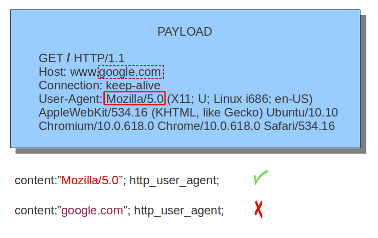
\includegraphics[scale=0.8]{user_agent_match.png}
    \caption{http.user\_agent keyword}
    \label{fig:user-agent}
\end{figure}


In questo progetto l'applicazione realizzata  inoltra su due diverse porte le richieste che 
provengono da un client che ha un sistema operativo Ubuntu e quelle che provengono da un 
client che ha un sistema operativo Windows. Per poter fare ciò nelle file delle firme 
(/tmp/signature.txt )ci sono due regole. La prima è quella rappresentata nell'esempio 4.2
e la seconda è quella presente nell'esempio 4.3.
Come abbiamo detto all'inizio della sezione le firme devono essere compilate e caricate nel 
motore regex. La successiva riga di comando effettua la prima operazione di compilazione.
La seconda operazione di caricamento la vedremo nel capitolo \ref{chapter:implementazione}

\begin{verbatim}
doca_dpi_compiler -i /tmp/signature.txt -o /tmp/signatures.cdo -f suricata
\end{verbatim}

\begin{table}[ht]
    \centering
    \caption*{\textbf{Esempio 4.5 } Regola Suricata per rilevare pacchetti provenienti da client Ubuntu}
    \begin{tabular}{ |l|c|}
        \hline
        alert http any any -> any any (msg:"pacchetto ricevuto da client Ubuntu;\\
        content:"Mozilla/5.0 (X11; Ubuntu; Linux x86\_64; rv:101.0)"; \\
        http\_user\_agent;sid:1)\\

        \hline
    \end{tabular}
\end{table}


\begin{table}[H]
    \centering
    
    \caption*{\textbf{Esempio 4.6} Regola Suricata per rilevare pacchetti provenienti da client Windows}
    \begin{tabular}{ |l|c|}
        \hline
        alert http any any -> any any (msg:"pacchetto ricevuto da client Windows"; \\
        content:"Mozilla/5.0 (Windows; U; Windows NT 5.1; en-US; rv:1.0.2)"; \\
        http\_user\_agent;sid:2)\\

        \hline
    \end{tabular}
\end{table}



%_________________________________________________________________________________________________

\section{Tabelle Hash}
\label{chapter:hash table}
Una volta ispezionato un pacchetto e stabilito lo user agent di provenienza e quindi anche la porta
su cui instradarlo, la cosa migliore è salvare queste informazioni in una struttura dati.
Così se si presenta un pacchetto proveniente dallo stesso client non c'è più la necessità di analizzarlo
nuovamente.Ma solamente cercare nella struttura dati la porta di uscita.
Come struttura dati abbiamo scelto le tabelle hash. per la loro efficienza.
Di seguito è riportato una piccola panoramica sulle tabelle hash (\cite{hash table }).

Un'hash table è una struttura dati usata per mettere in corrispondenza una data chiave con un 
dato valore.

\begin{figure}[h]
    \centering
    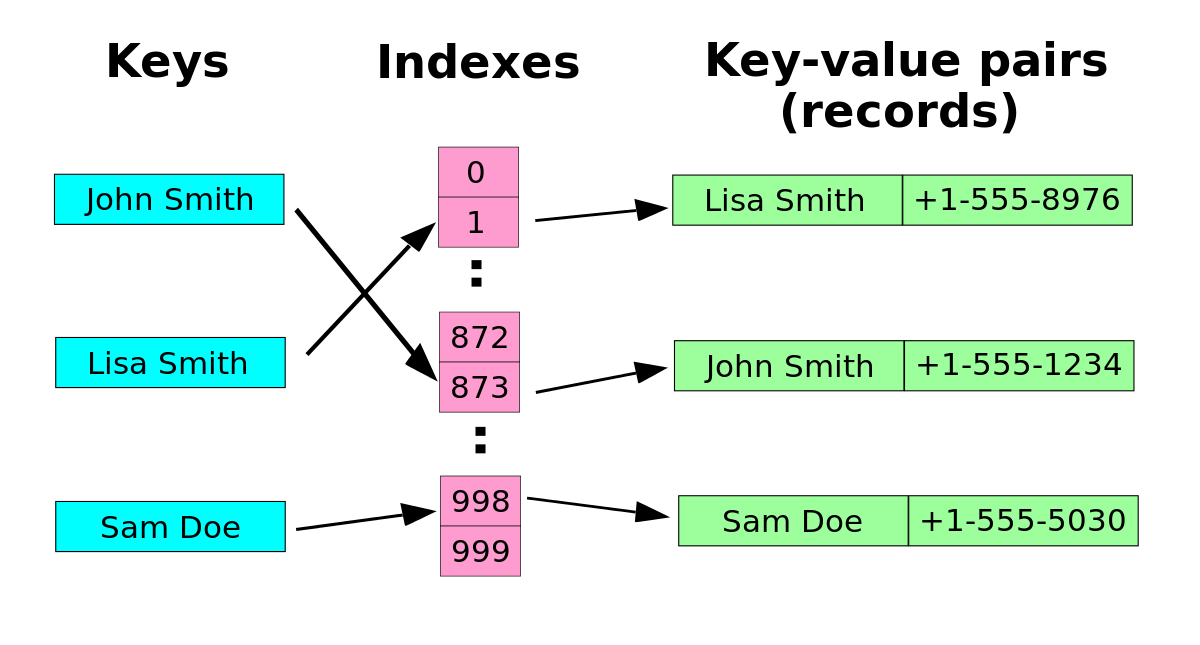
\includegraphics[scale=0.2]{hash-table.png}
    \caption{Hash table}
    \label{fig:hash-table}
\end{figure}

È molto utilizzata nei metodi di ricerca nominati hashing ovvero un'estensione 
della ricerca indicizzata da chiavi che gestisce problemi di ricerca nei quali le chiavi di 
ricerca non presentano queste proprietà. Una ricerca basata su hashing è completamente diversa 
da una basata su confronti: invece di muoversi nella struttura data in funzione dell'esito dei 
confronti tra chiavi, si cerca di accedere agli elementi nella tabella in modo diretto tramite 
operazioni aritmetiche che trasformano le chiavi in indirizzi della tabella. 

Esistono vari tipi di algoritmi di hashing. Per quanto affermato, in una tabella di hashing 
ben dimensionata il costo medio di ricerca di ogni elemento è indipendente dal numero di elementi.
L'hashing è un problema classico dell'informatica; molti algoritmi sono stati proposti, studiati
a fondo e impiegati in pratica. Due metodi molto diffusi sono l'hashing statico e l'hashing 
estendibile e lineare, metodi utilizzati anche dai programmi DBMS. 

Il primo passo per realizzare algoritmi di ricerca tramite hashing è quello di determinare 
la funzione di hash: il dato da indicizzare viene trasformato da un'apposita funzione di hash 
in un intero compreso tra $0 $ ed $m-1$ 
che viene utilizzato come indice in un array di lunghezza $m$. Supponendo che $U$
sia l'universo delle chiavi e $T [0... m-1]$  una tabella 
hash, una funzione hash $h$, stabilisce una corrispondenza tra $U$ e le posizioni
nella tabella hash, quindi:
\begin{displaymath}
    h:U \to \{0,1,...,m-1\}
\end{displaymath}

Idealmente, chiavi diverse dovrebbero essere trasformate in indirizzi differenti, 
ma poiché non esiste la funzione di hash perfetta, ovvero totalmente iniettiva,
è possibile che due o più chiavi diverse siano convertite nello stesso indirizzo.
Il caso in cui la funzione hash applicata a due chiavi diverse genera un medesimo 
indirizzo viene chiamato collisione e può essere gestito in vari modi.
La scelta di una buona funzione di hash è indispensabile per ridurre al minimo 
le collisioni e garantire prestazioni sempre ottimali. Il risultato migliore
si ha con funzioni pseudo-casuali che distribuiscono i dati in input in modo uniforme. 

Molto spesso però, una buona funzione di hash può non bastare: infatti le prestazioni 
di una hash table sono fortemente legate anche al cosiddetto fattore di carico (load factor)
calcolato come $   \frac{\text{cardinalità insieme di chiavi da inserire}}{\text{dimensione massima della struttura} }$ 
e che dice quanta probabilità ha un nuovo elemento di collidere con uno già presente nella tabella.
Questa probabilità, in realtà, è più alta di quanto si possa pensare, come dimostra il 
paradosso del compleanno. È bene dunque mantenere il load factor il più basso possibile
(di solito un valore di 0.75 è quello ottimale) per ridurre al minimo il numero di collisioni. 
Ciò può essere fatto, ad esempio, ridimensionando l'array ogni volta che si supera il load 
factor desiderato. 


Nel nostro progetto, nell'hash table vengono salvate le coppie 5-tupla/ porta di uscita.
Una 5-tupla come monstrato nella tabella \ref{tab:5-tupla} è composta dall'indirizzo Ip sorgente,
la porta sorgente, l'indirizzo Ip destinazione,la porta di destinazione ed il protocollo.
Questi 5 parametri identificano una sessione TCP/UDP.


\begin{table}[H]
    
    \caption{Esempio di una 5-tupla di un pacchetto}
    \footnotesize
    \begin{tabular}{|c |c |c |c|c|} 
     \hline
     \textbf{Ip sorgente} & \textbf{porta sorgente} & \textbf{Ip destinazione} & \textbf{porta destinazione} & \textbf{protocollo} \\ 
     \hline
     192.168.100.200 & 34406 & 128.119.245.12 & 80 & 6\\ 
     \hline
    \end{tabular}
    \label{tab:5-tupla}
    

\end{table}
La porta di uscita invece è la porta sulla quale il load balancer inoltrerà il pacchetto.
Nella figura \ref{fig:hash-table-5-tuple} è rappresentata l'hash table utilizzata 
nell'implementazione
\begin{figure}[h]
    \centering
    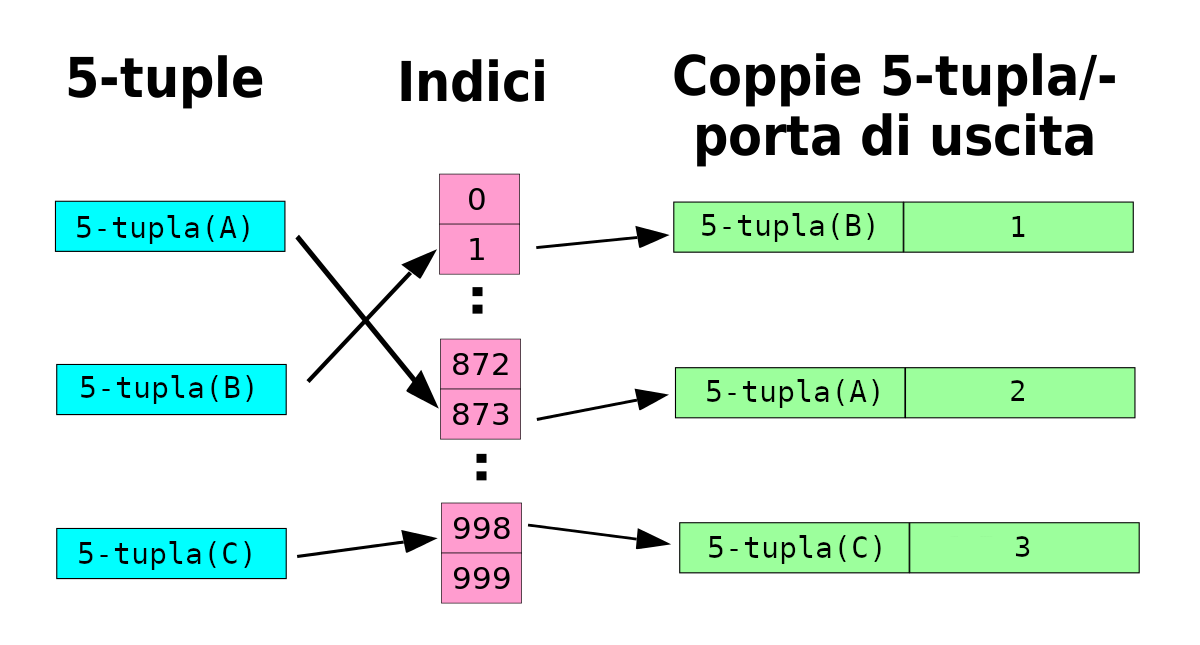
\includegraphics[scale=0.24]{hash-table-5-tuple.png}
    \caption{Tabella hash 5-tuple/porta di uscita}
    \label{fig:hash-table-5-tuple}
\end{figure}

%_________________________________________________________________________________________________
\section{Implementazione}
\label{chapter:implementazione}

In questa sezione vedremo l'implementazione dell'applicazione descrivendo l'algoritmo e alcune
funzioni più importanti.L'intero progetto è reperibile sulla pagina 
Github(\url{https://github.com/sup3rbu/load_balancer-bluefield-prototype})
\subsubsection*{Algoritmo}

\begin{tabular}{c}
    \hline
\begin{lstlisting}[basicstyle=\normalsize,  frame=none,firstnumber=0    ]
inizializza();
buffer <- recupera_pacchetti();
for pacchetto in buffer 
    tupla <- estrai_tupla(pacchetto);
    h <- hash(tupla);
    if (TabellaHash.contieneChiave(h) )
        porta_di_uscita <- TabellaHash.ottieni(h);
    else 
        porta_di_uscita < calcola_porta_uscita(pacchetto);
        hashtable <-TabellaHash.inserisci(h,porta_di_uscita).
    inoltra_pacchetto(pacchetto,porta_di_uscita);

\end{lstlisting}\\
\hline
\end{tabular}\\
\\\\
In questo algoritmo vediamo diversi passi del programma.
Il primo è l'inizializzazione che comprende l'inizializzazione di dpdk ,il caricamento del
file del firme compilato (/tmp/signature.cdo), l'inizializzazione della
libreria DOCA Dpi e la creazione dell'hash table.\\
Poi abbiamo la funzione recupera\_pacchetti() che sarebbe la corrispettiva funzione dpdk
rte\_eth\_rx\_burst()  che recupera una raffica di pacchetti di input da una coda di ricezione di
un dispositivo Ethernet e li archivia in un buffer.\\
Dopodiché per ogni pacchetto in entrata viene controllato se la rispettiva 5-tupla è presente nella tabella
hash. Se è presente, estraimo la porta di uscita ed inoltriamo il pacchetto.
Se non è presente richiamiamo la funzione calcola\_porta\_uscita() (nel codice dpi\_scan) che controlla lo user agent e determina
in base a quest'ultimo campo la porta di uscita.



\subsubsection*{Funzioni principali}
Tra le funzioni principali del programma abbiamo il main().


\begin{lstlisting}[title= int main();, language=C,firstnumber=69]
int main(int argc, char **argv)
{
	struct application_dpdk_config dpdk_config = {
		.port_config.nb_ports = 2,
		.port_config.nb_queues = 2,
		.port_config.nb_hairpin_q = 4,
		.sft_config = {0},
	};

	/* init and start parsing */
	struct doca_program_general_config *doca_general_config;
	struct doca_program_type_config type_config = {
		.is_dpdk = true,
		.is_grpc = false,
	};

	/* Parse cmdline/json arguments */
	arg_parser_init("dns_filter", &type_config, NULL);
	arg_parser_start(argc, argv, &doca_general_config);

	struct rte_hash *hashtable;
	ut_params.name = "test1";
	hashtable = rte_hash_create(&ut_params);
	if (hashtable == NULL)
		rte_panic("Failed to create cdev_map hash table, errno = %d\n", rte_errno);

	/* update queues and ports */
	dpdk_init(&dpdk_config);

	load_balancer_init();

	scan(dpdk_config.port_config.nb_queues, dpdk_config.port_config.nb_ports, hashtable);

	return 0;
}
\end{lstlisting}
Poi la funzione scan() che recupera i pacchetti di input da una coda
di ricezione di un dispositivo Ethernet. Il buffer ottenuto viene passato come parametro alla 
funzione handle\_packets\_received();

 


\begin{lstlisting}[title=handle\_packets\_received();, language=C,firstnumber=170]
for (current_packet = 0; current_packet < packets_received; current_packet++)
	{

		sid = 0;
		uint32_t payload_offset = 0;
		struct rte_sft_mbuf_info mbuf_info = {0};
		struct doca_dpi_parsing_info parsing_info = {0};
		struct rte_sft_error error;

		packet = packets[current_packet];

		rte_sft_parse_mbuf(packet, &mbuf_info, NULL, &error);
		set_l4_parsing_info(&parsing_info, &payload_offset, &mbuf_info);

		extract_tuple(&tuple, parsing_info);
		print_tuple(tuple);

		ret = rte_hash_lookup_data(hashtable, &tuple, (void **)&sid);

		if (ret == -ENOENT)
		{
			//DOCA_LOG_INFO("tupla non presente");
			DOCA_LOG_INFO("DPI scan");
			sid = dpi_scan(packet, &parsing_info, &payload_offset);
			if (sid)
				ret = rte_hash_add_key_data(hashtable, &tuple, (void *)sid);
		}
		else
		{
			//DOCA_LOG_INFO("tupla presente valore:%d", sid);
		}


		if (sid == 1)
			egress_port = packet->port ^ 1;
		else
			egress_port = packet->port;

		rte_eth_tx_burst(egress_port, queue_id, &packets[current_packet], 1);
	}
\end{lstlisting}

Infine un'ultima funzione importante è la dpi\_scan();
Che processa il contenuto del pacchetto , controlla se c'è un riscontro con 
le firme caricate nel motore Regex e se c'è ritorna il SID(signature id), così sappiamo
da quale dispositivo proviene il pacchetto.
\newpage


\begin{lstlisting}[title= dpi\_scan();, language=C,firstnumber=236]
int dpi_scan(struct rte_mbuf *packet, struct doca_dpi_parsing_info *parsing_info,
			 uint32_t *payload_offset)
{
	bool to_server = true;
	int err, ret;
	int packets_to_process = 0;
	uint16_t dpi_queue = 0;
	struct doca_dpi_sig_data sig_data;
	struct doca_dpi_flow_ctx *flow_ctx = NULL;
	struct doca_dpi_result result = {0};
	struct doca_dpi_stat_info stats = {0};
	/* Create DPI flow according to packet info */
	flow_ctx = doca_dpi_flow_create(dpi_ctx, dpi_queue, parsing_info, &err, &result);
	if (err < 0)
	{
		DOCA_LOG_ERR("DPI flow creation failed, error=%d", err);
		return err;
	}

	ret = doca_dpi_enqueue(flow_ctx, packet, to_server, *payload_offset, NULL);
	if (ret == DOCA_DPI_ENQ_PROCESSING || ret == DOCA_DPI_ENQ_BUSY)
		packets_to_process = 1;
	else if (ret < 0)
	{
		DOCA_LOG_ERR("DPI enqueue failed, error=%d", ret);
		return ret;
	}

	while (packets_to_process > 0)
	{
		if (doca_dpi_dequeue(dpi_ctx, dpi_queue, &result) == DOCA_DPI_DEQ_READY)
		{
			packets_to_process -= 1;
			if (result.matched)
			{
				ret = doca_dpi_signature_get(dpi_ctx, result.info.sig_id,
											 &sig_data);
				if (ret < 0)
				{
					DOCA_LOG_ERR("Failed to get signatures - error=%d", ret);
					return ret;
				}
				DOCA_LOG_INFO(
					"DPI found a match on signature with ID: %u and URL MSG: %s\n",
					result.info.sig_id, sig_data.name);
			}
		}
	}

}

\end{lstlisting}

%_______________________________________________________________________________________________
\chapter{Conclusione}
Alla fine di questo elaborato riassiumiamo tutto il lavoro e lo studio svolto in questo tirocinio.

Abbiamo visto cosa sono le data processing unit, questa nuova tipologia di processori che 
gesticono lo spostamento delle informazioni nei data center e che liberano le CPU dai carichi
di lavoro di rete e di comunicazione.

Poi abbiamo visto la DPU Nvidia Bluefield-2 , le sue caratterische tecniche ,i suoi 
acceleratori hardware ed il suo kit di sviluppo DOCA.\\
Abbiamo sfruttato il suo motore Regex. Un motore di espressioni regolari
che si occupa di elaborare la corrispondenza dei pattern per i payload dei pacchetti rete.

Abbiamo realizzato un load balancer che agisce al livello 7 della pila OSI.
Un'applicazione che instrada i pacchetti in base a determinati campi del protocollo HTTP.




%_______________________________________________________________________________________________

\backmatter
%\cleardoublepage
%\let\cleardoublepage\clearpage
  
\addcontentsline{toc}{chapter}{\bibname}

\begin{thebibliography}{9}
\bibitem{What Is a DPU}
"What Is a DPU?And what’s the difference between a DPU, a CPU and a GPU?"


\url{https://blogs.nvidia.com/blog/2020/05/20/whats-a-dpu-data-processing-unit/}

\bibitem{BLUEFIELD-2 DPU DATASHEET}
NVIDIA BLUEFIELD-2 DPU DATASHEET

\url{https://resources.nvidia.com/en-us-accelerated-networking-resource-library/bluefield-2-dpu-datasheet?lx=LbHvpR&topic=networking-cloud}

\bibitem{DPU Modes of Operation}
NVIDIA BlueField DPU Modes of Operation

\url{https://docs.nvidia.com/doca/sdk/modes-of-operation/index.html}

\bibitem{Reti di calcolatori}
Reti di calcolatori e internet. Un approccio top-down.
James F. Kurose. Keith W. Ross

\url{https://www.amazon.it/calcolatori-internet-approccio-top-down-aggiornamento/dp/8891902543}

\bibitem{documentazione Suricata}
Documentazione Suricata

\url{https://suricata.readthedocs.io/en/suricata-6.0.0/rules/intro.html}
\bibitem{doca doc url filter}
DOCA Installation guide ;DOCA URL-Filter

\url{https://docs.nvidia.com/doca/archive/doca-v1.2.1/installation-guide/index.html}\\
\url{https://docs.nvidia.com/doca/archive/doca-v1.2.1/url-filter/index.html}

\bibitem{doca doc scalable function }
DOCA Scalable Function

\url{https://docs.nvidia.com/doca/sdk/scalable-functions/index.html}

\bibitem{hash table }
Hash table Wikipedia

\url{https://it.wikipedia.org/wiki/Hash_table}
\bibitem{install bluefield }
NVIDIA Mellanox Bluefield-2 SmartNIC Hands-On Tutorial: “Rig for Dive” — Part I: Install Drivers and Access the SmartNIC

\url{https://medium.com/codex/getting-your-hands-dirty-with-mellanox-bluefield-2-dpus-deployed-in-cloudlabs-clemson-facility-bcb4e689c7e6}



\end{thebibliography}  
% Here put the code for the bibliography. You can use BibTeX or
% the BibLaTeX package or the simple environment thebibliography.
\end{document}


%cose da aggiungere:
% -1 la compilazione delle firme (compiler signature.txt -> signature.cdo)
% -2 file di build meson ...
% -3
% -4
% -5